\documentclass{csfourzero}

\author{Philip Hale}
\title{A comparison of developments in PSO from 1995 to 2013}

\usepackage[utf8]{inputenc} % allows UTF-8 in references
\usepackage{natbib} % support for alpha style
\usepackage{amsmath} % better rendering of formulae
\usepackage{graphicx} % graphics support
\usepackage{epstopdf} % eps support
\usepackage{multicol} % multiple columns
\usepackage{caption} % helps with multicol + figures
\usepackage{siunitx} % easier to use and read standard form. E.g. \num{3e-2}
\sisetup{tight-spacing=true}

% Sort-of chicago-style (humanities) inline references.
\bibliographystyle{alpha}

% aligns overrightarrows in math formulae
\newcommand{\rarrow}[1]{\overrightarrow{#1\vphantom{b}}}

% sensible figures in multi-column environments
\newenvironment{Figure}
  {\par\medskip\noindent\minipage{\linewidth}}
  {\endminipage\par\medskip}

\begin{document}

\maketitle

\section{Abstract}

This paper compares the gold-standard of Particle Swarm Optimization
(SPSO-2011) with a canonical PSO implementation that is similar to original
designs from 1995. The success of each algorithm is determined by its ability
to optimize 4 functions. We begin by introducing PSO and the differences
between the algorithms under test, and conclude by evaluating the extent to
which limitations of PSO have been addressed by the current standard.

\section{Introduction}

Particle Swarm Optimization is a comparatively new evolutionary computation
technique, having only been around since 1995.  Conceptually the algorithm
emulates a flock of birds circling a roost, resulting in  behaviour described
by the original paper as ``flying potential solutions through hyperspace,
accelerating toward `better' solutions''~\cite{Kennedy:1995bi}.

Since the algorithm is simple and competitive with more complex and mature
optimization techniques, it has been the subject of much study. Research has
been primarily concerned with avoiding the potential for the algorithm to
prematurely converge on a non-global minima, and increasing the speed at which
convergence occurs~\cite{vandenBergh:2002tk}.

In 2007~\cite{Bratton:2007hq}, and then again in 2011~\cite{Clerc:2012to}, a
Standard PSO (SPSO) was proposed in order to give future research a baseline
comparison. Prior to this date, much of the claimed improvements to PSO were
made by comparison with an outdated model of PSO that didn't reflect a fair
baseline. This made comparison between results difficult. The new standards
provide a benchmark that mean  ``if your brand new algorithm does not
significantly `beat' SPSO (on a difficult enough non-biased benchmark) you have
to improve it''~\cite{Clerc:2012to}.

SPSO is not meant to be outperform every flavour of PSO either generally or on a
subset of optimization targets~\cite{Bratton:2007hq}. More performant PSO
implementations exist, but the improvements are either still under scrutiny or
limited to certain classes of functions.

Comparing the contemporary baseline-performance of PSO with an implementation
that resembles PSO from the late nineties allows us to assess how far the field
has come, and to what extent some of PSO's earlier limitations are still
relevant.

\section{PSO Variants under Test}

\subsection{Original PSO}

The algorithm consists of a population of particles, where each particle
represents a candidate solution to the objective function.  The number of
particles is referred to as the swarm-size, and is notated by $S$.

The dimension of the search space $D$ determines the magnitude of the position
and velocity matrices for each particle. Formally, the $position$ and $velocity$
for the $i^{th}$ particle are denoted by
$\rarrow{X_i} = x_{i1}, x_{i2},\ldots,x_{iD}$ and
$\rarrow{V_i} = v_{i1}, v_{i2},\ldots,v_{iD}$ respectively.
Initialization takes place by giving each particle a random velocity and
position within the search space.

Each particle keeps track of the best position they have reached so far. This is
known as the $personal best$, and is represented by $\rarrow{P_i} = p_{i1}, p_{i2},\ldots,p_{iD}$.
The performance or `fitness' of a given position can be determined by evaluating
the objective function with the position values as input. After each iteration,
the global best $g$ is updated with the best position of all particles in the
swarm.

Each iteration of the algorithm updates each particle's velocity and position.
These are computed as follows:

\begin{equation} \label{eq:orig_v_update}
\rarrow{V}_i^{t+1} = \rarrow{V}_i^t + c_1 \rarrow{U}_1^t \circ (\rarrow{P}_i^t - \rarrow{X}_i^t) + c_2 \rarrow{U}^t_2 \circ (g^t - \rarrow{X}_i^t)
\end{equation}

\begin{equation} \label{eq:orig_p_update}
\rarrow{X}_i^{t+1} = \rarrow{X}_i^t + \rarrow{V}_i^{t+1}
\end{equation}

$t = 1, 2,\ldots,T$, where T is the number of iterations. $c_1$ and $c_2$ are
the $cognitive$ and $social$ weights used to control the bias between locally
optimized and globally optimized search. $\rarrow{U}_1$ and $\rarrow{U}_2$ are
random vectors in the range $[0,1]$, and $\circ$ denotes the Hadamard product,
also known as entrywise product, of the two matrices.

Variations of the PSO algorithm consist of changes in the initialization of the
swarm, modifications to the velocity and positional update functions. These
are explained in detail below in defining the two algorithms under test.

\subsection{Canonical PSO}

Early analysis of the original PSO algorithm revealed some limitations, chief
among them premature convergence~\cite{vandenBurgh:2002tk} and a comparatively
slow convergence speed~\cite{Shi:1998kl}. Alterations to the original approach
were suggested, and since some of these advancements have been present for a
decade or more, they have been included in this specification of Canonical
PSO\@.

The modifications described below have the effect of changing the velocity
update equation to:

\begin{equation} \label{eq:canon_v_update}
\rarrow{V}_i^{t+1} = \omega \rarrow{V}_i^t + c_1 \rarrow{U}_1^t \circ (\rarrow{P}_i^t - \rarrow{X}_i^t) + c_2 \rarrow{U}^t_2 \circ (\rarrow{L}^t - \rarrow{X}_i^t)
\end{equation}

%\subsubsection{In summary}

%\begin{description}
  %\item[Type] local-best (with neighbourhoods)
  %\item[Vmax] Range of search space
  %\item[Initial velocity] Random between $-Vmac$ and $Vmax$
  %\item[Initial position] Randomly around the unshifted center of the function
  %\item[Topology] Ring-topology
  %\item[Peers per neigbourhood] 10
  %\item[Inertia] Linear decreasing from 0.9 to 0.4
  %\item[$c_1$] 1.49618
  %\item[$c_2$] 1.49618
%\end{description}

\subsubsection{Inertia Weight}

Upon closer examination of the original PSO update procedure, it can be seen
that the cognitive and social weight values determine whether the search-space
contracts towards a best-known minimum or expands to explore a new range of
solutions. Given this tradeoff, it makes sense to introduce a new parameter that
``plays the role of balancing the global search and local search''. This is
called the inertia weight~\cite{Shi:1998kl}. Empirical evidence has suggested
that a linear-decreasing inertia weight gives the best results, where the
initial linear weight of $0.9$ decreases to $0.4$ as the number of iterations
increases~\cite{Shi:1998jj}.

This introduces a new parameter $\omega$ to the velocity update equation, which
gives momentum to the current velocity.

\subsubsection{Local Best; Neighbourhoods}

The specification above describes $\text{global best}$ or $gbest$ PSO\@. This
has the unfortunate property of premature convergence. In fact, until Guaranteed
Convergence PSO was introduced~\cite{vandenBergh:2002tk}, the algorithm could
not even guarantee convergence on a local minima.

A solution was proposed in the form of $local best$ or $lbest$ PSO, which groups
the particles into distinct neighbourhoods, each with their own best-so-far
position value~\cite{Sugunthan:1999iv}. Instead of a globally-known best
solution, each neighbourhood has its own local-best position. Earlier versions
of PSO were characterised by using this $lbest$ variation, and so it has been
chosen for the comparison. The paper that first proposed $lbest$ PSO used
Eculidian distance to determine neighbourhood groupings.  Canonical PSO uses the
more popular and computationally cheaper ring topology, which creates
neighbourhoods based on the array index of the particle swarm.

This has the effect of changing the algorithm such that instead
of a global best $g$, the best-known position of a particle's neighbourhood is
represented by $\rarrow{L} = l_1, l_2,\ldots,l_D$.

\begin{multicols}{3}
  \begin{Figure}
    \centering
    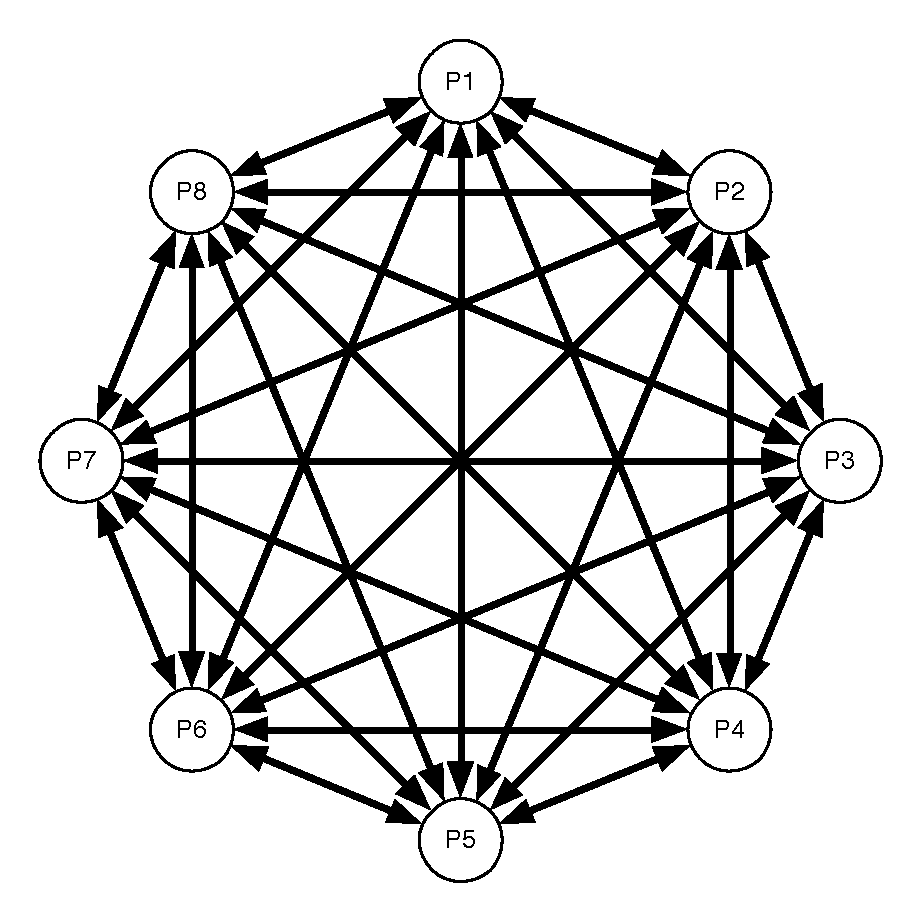
\includegraphics[width=\linewidth]{global_best_topology.eps}\label{fig:global_best_topology}
    \captionof{figure}{Global-best topology}
  \end{Figure}

  \begin{Figure}
    \centering
    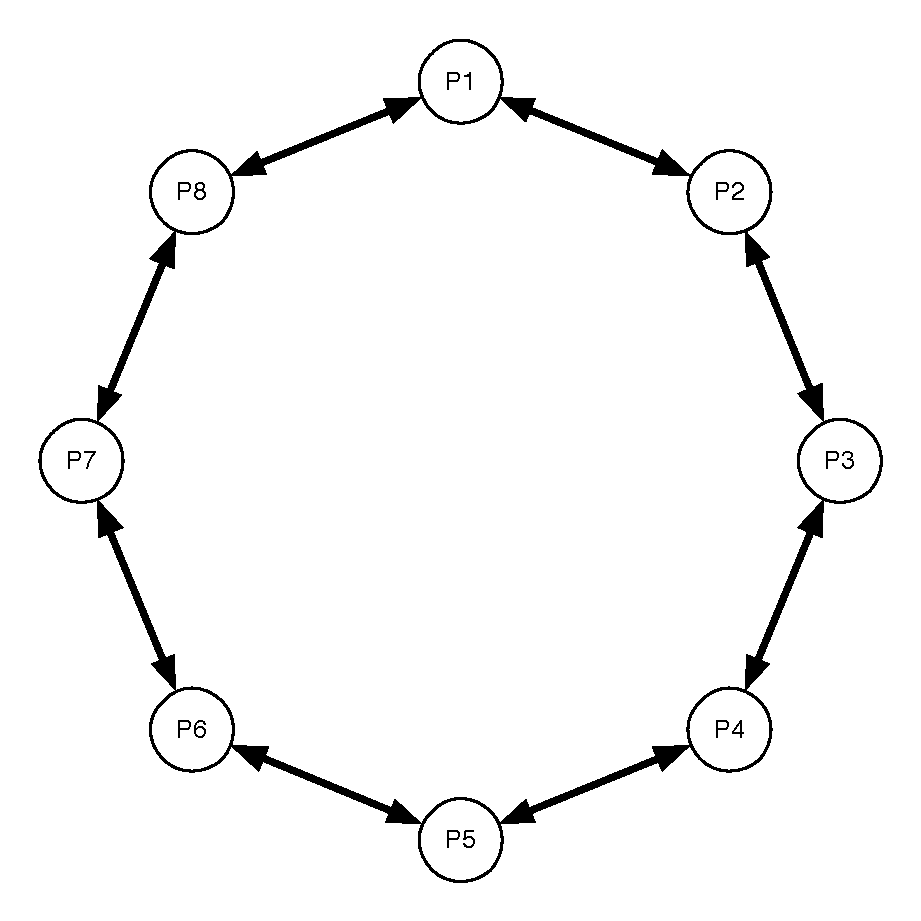
\includegraphics[width=\linewidth]{ring_topology.eps}\label{fig:ring_topology}
    \captionof{figure}{Ring topology}
  \end{Figure}

  \begin{Figure}
    \centering
    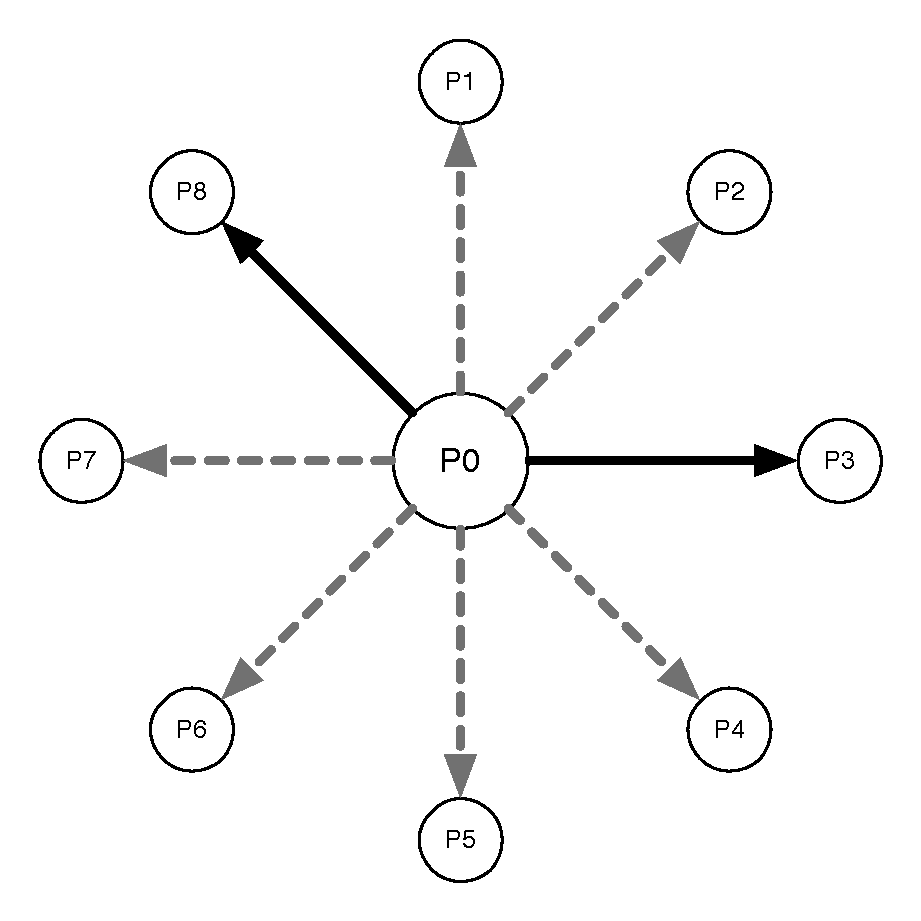
\includegraphics[width=\linewidth]{star_topology.eps}\label{fig:adaptive_random_topology}
    \captionof{figure}{Adaptive-random topology}
  \end{Figure}
\end{multicols}

\subsection{SPSO 2011}

The effect of the modifications below is this new velocity-update formula, where
$H_i(\rarrow{G}_i^t,||\rarrow{G}_i^t - \rarrow{X}_i^t||)$ describes the
hypersphere:

\begin{equation}
  \rarrow{V}_i^{t+1} = \omega \rarrow{V}_i^t + H_i(\rarrow{G}_i^t,||\rarrow{G}_i^t - \rarrow{X}_i^t||) - \rarrow{X}_i^t
\end{equation}


\subsubsection{Initialisation of the swarm}

Like Canonical PSO, the initial position of particles is randomised within the
search space. Unlike Canonical PSO, the velocity is determined by:

\begin{equation}
  V_i^0 = U(D_{min} - X_i^d, D_{max} - X_i^d)
\end{equation}

In addition, the parameter values are normalised, which transforms the
search-space into a hypercube. This is in order to gain maximum benefit from the
new velocity update equation, which makes use of
hyperspheres~\cite{Clerc:2012to}.

\subsubsection{Neighbourhood}

Like Canonical PSO, SPSO-2011 also supports neighbourhoods. However whereas
Canonical PSO groups neighbours in a ring
topology~(Figure~\ref{fig:ring_topology}), SPSO-2011 implements adaptive-random
topology~(Figure~\ref{fig:adaptive_random_topology}). This introduces
variability into the neighbourhoods, whereby the neighbourhood changes each time
the local-best score stays the same.

With the suggested parameters, this means each particle informs itself plus a
maximum of two other randomly selected particles. By implication each particle
can be informed by anything from just itself to every particle in the swarm,
since a particle can be chosen more than once. In other words, ``the information
of the location of the global best is only communicated to a subset of the
swarm, and the composition of this subset varies from iteration to
iteration''~\cite{Miranda:2007er}

\subsubsection{Velocity update equations}

SPSO-2011 addresses a long running concern in PSO analysis, where functions that
have minimums on the axis of the search space are much easier to optimize. The
technique to address this requires using rotational invariance to perform the
calculation based on a point slightly skewed from the known positions. The
effect of this operation is a more uniform distribution of all next possible
positions, $DNPP$.  This process and its effects are explained more thoroughly
in~\cite{ZambranoBigiarini:2013dl}.

\begin{multicols}{2}

\begin{Figure}
  \centering
  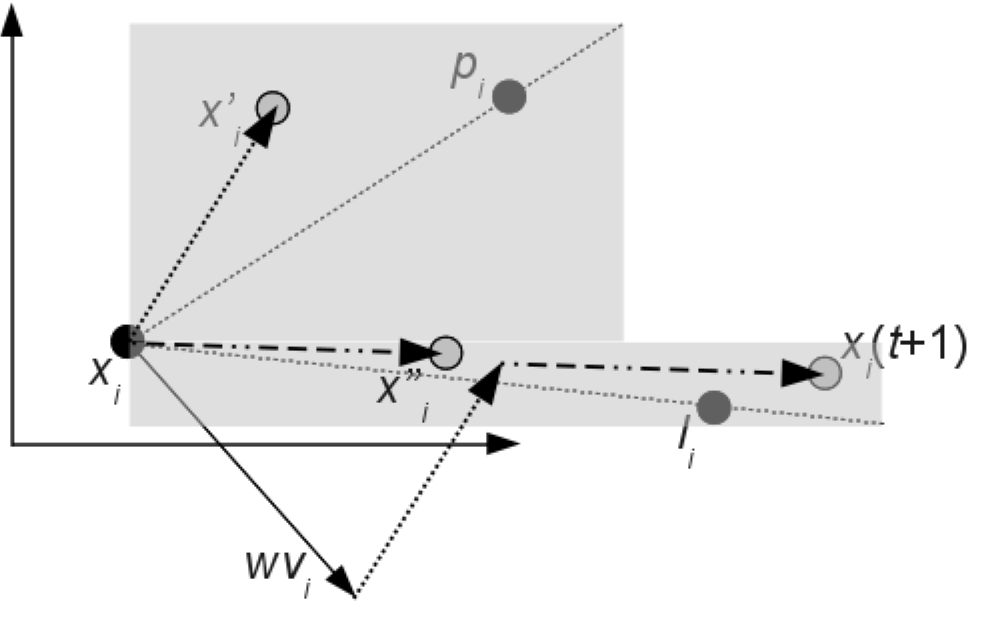
\includegraphics[width=0.8\linewidth]{dnpp_canonical.png}\label{fig:dnpp_canonical}
  \captionof{figure}{DNPP in Canonical PSO, adapted from~\cite{ZambranoBigiarini:2013dl}}
\end{Figure}

\begin{Figure}
  \centering
  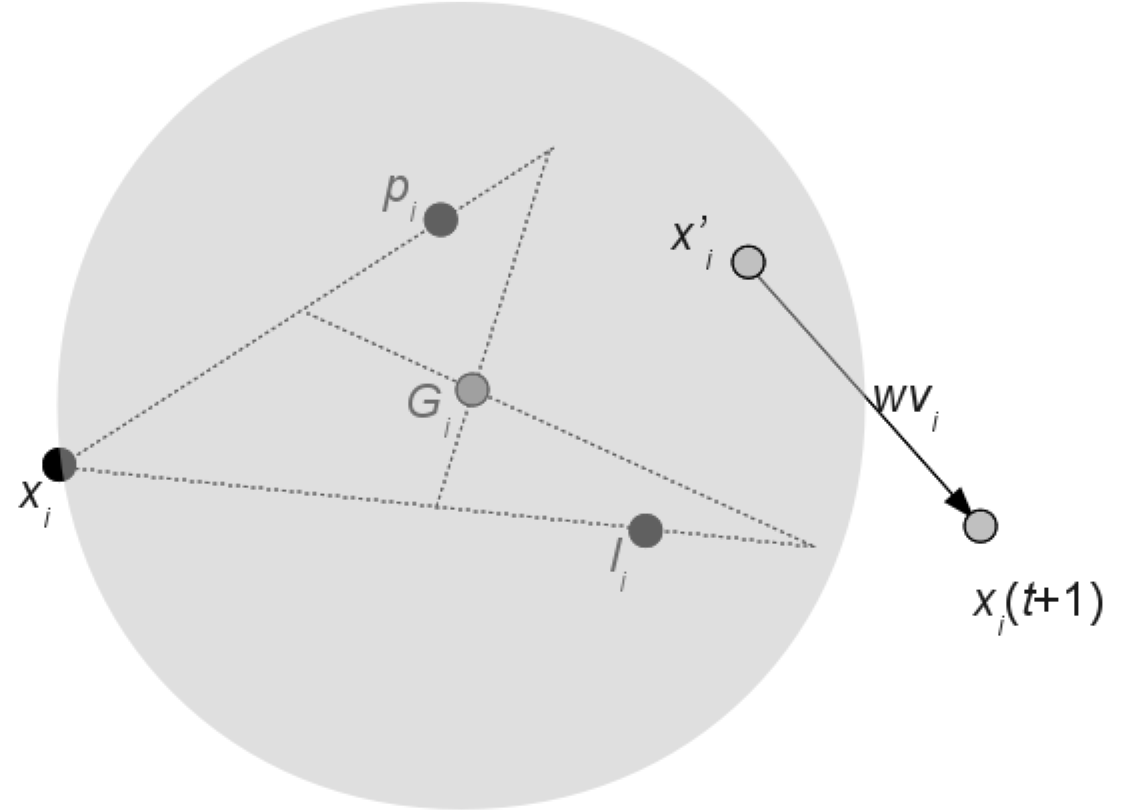
\includegraphics[width=0.8\linewidth]{dnpp_spso11.png}\label{fig:dnpp_spso11}
  \captionof{figure}{DNPP in SPSO-2011, adapted from~\cite{ZambranoBigiarini:2013dl}}
\end{Figure}

\end{multicols}

\subsubsection{Confinement} % aka velocity clamping

``When a particle `flies' outside the $[min_d ,max_d]$ range, each boundary of
the search space acts as an absorbing wall, modifying the position of the
particle to coincide with the reached boundary and resetting the particle's
velocity to zero.''~\cite{ZambranoBigiarini:2013dl}.

\subsection{Commonalities between both PSO variations under test}

Some parameters have been kept the same between the variations under test, for
two reasons. Firstly, because the parameter values do not represent a
fundamental advancement of the algorithm, and so it makes sense to set them to
best known values. Secondly, to ensure that the comparison is accurate and does
not unfairly bias one approach due to parameter choice rather than a genuine
development of the algorithm.

\subsubsection{Swarm size}

It is not currently known how to pick the optimal number of particles (Trelea
2003), so a medium value of 40 has been chosen. Increasing the swarm size
increases the success rate at the expense of function evaluations. Since our
stopping criteria in this simulation is a set number of function evaluations,
it is important that the swarm size remains constant for both algorithms.


\section{Functions}

In order to overcome potential bias, the functions have been shifted such that
the particles are not initialized around the global
minimum~\cite{Monson:2005fn}.

Plots of the functions are 2-dimensional, with the z-axis representing the
function evaluation or fitness value for the given (x,y) positional coordinate.

%The Rosenbrock function is a widely test function in optimization. PSO was first
%tested against it in~\cite{Shi:1999je}, with an algorithm somewhat similar to
%the Canonical PSO described here.

\begin{multicols}{2}

\begin{Figure}
  \centering
  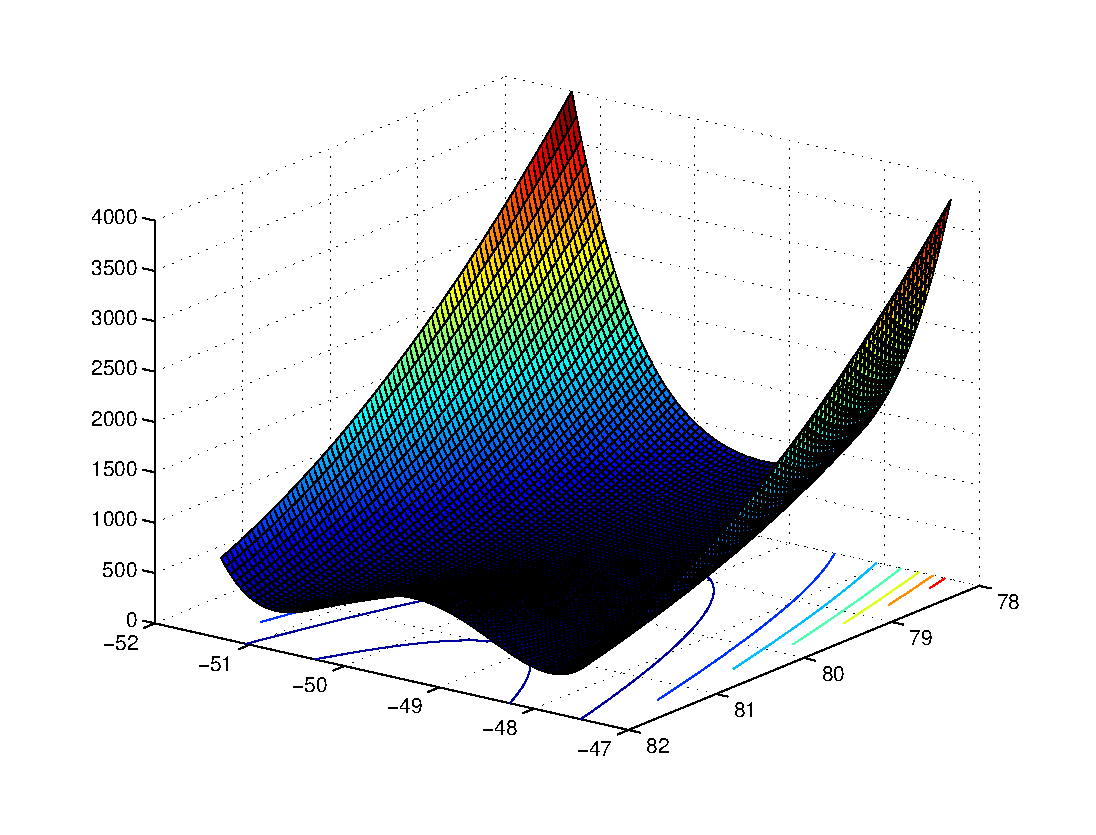
\includegraphics[width=\linewidth]{../functions/rosenbrock_shifted.eps}
  \captionof{figure}{Rosenbrock Function}
\end{Figure}

\begin{Figure}
  \centering
  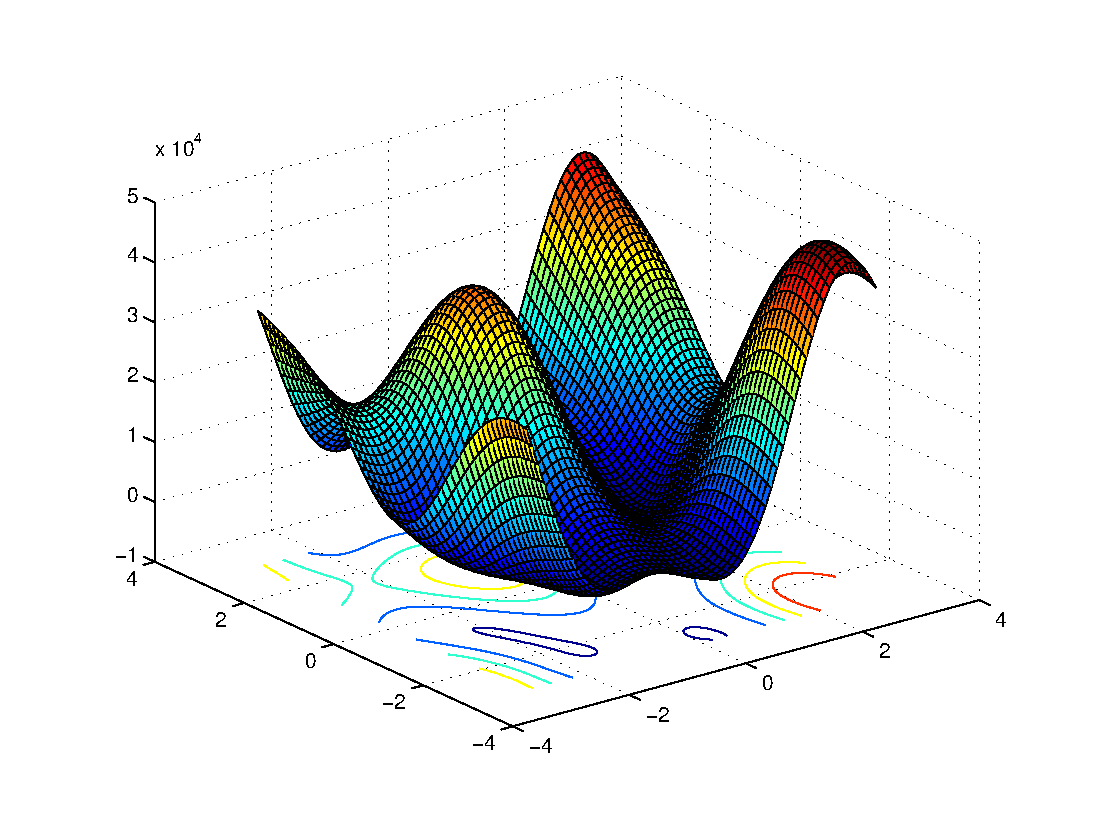
\includegraphics[width=\linewidth]{../functions/schwefel.eps}
  \captionof{figure}{Schwefel Function}
\end{Figure}

\begin{Figure}
  \centering
  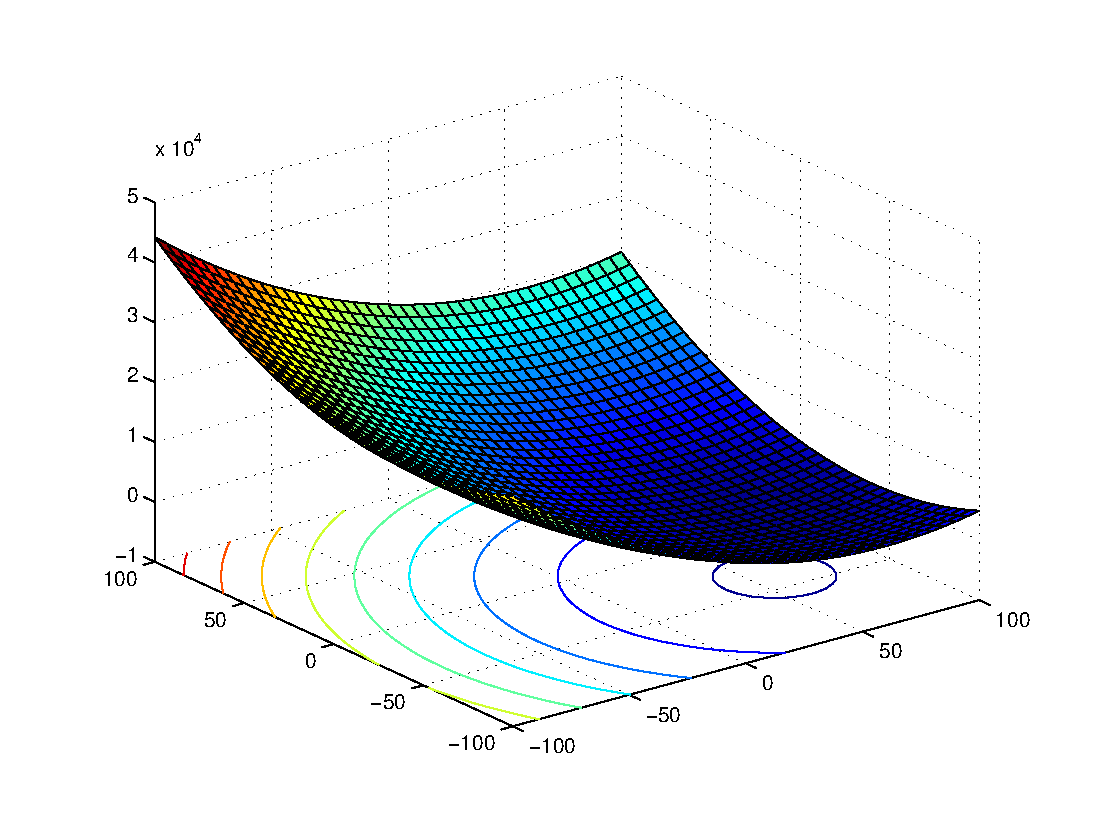
\includegraphics[width=\linewidth]{../functions/sphere_shifted.eps}
  \captionof{figure}{Sphere Function}
\end{Figure}

\begin{Figure}
  \centering
  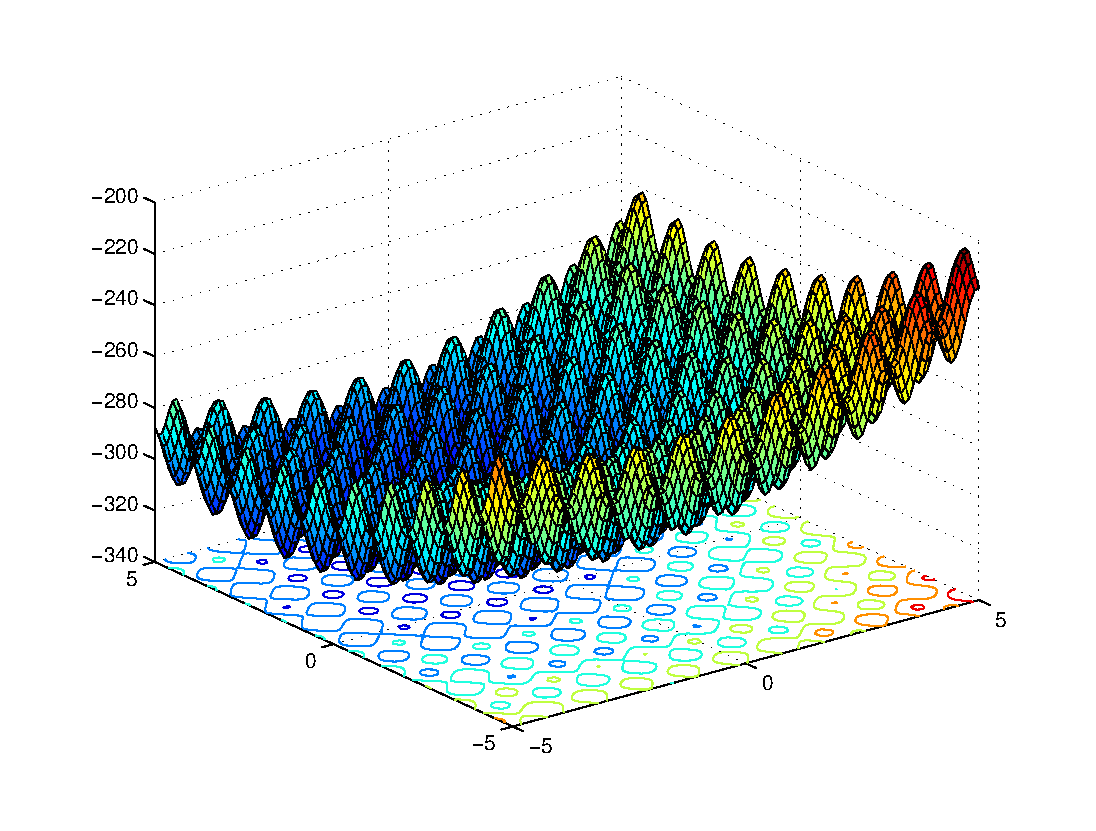
\includegraphics[width=\linewidth]{../functions/rastrigin_shifted.eps}
  \captionof{figure}{Rastrigin Function}
\end{Figure}

\end{multicols}

\section{Experimental Setup}

\subsection{Functions}

Separate results are given for runs carried out in 2 and 30 dimensions.

\subsection{Parameter selection}

In addition to and as a result of the differences in approach outlined above,
SPSO-2011 and Canonical PSO have different parameters.  This section lists the
setup for each PSO variation.

Four objective functions widely used in optimizatin literature have been tested
against, the results of which appear below. Two sets of results are presented,
against functions in 2 and 30 dimensions.

The maximum number of function evaluations is dependent on the number of
dimensions. This is in keeping with other PSO testing and allows for better
comparisons.

\subsubsection{Canonical PSO}
\begin{description}
  \item[Swarm size] 30
  \item[Particles per neighbourhood] (40/3) $\approx$ 13
  \item[Number of runs] 25
  \item[Maximum function evaluations] \num{1e5} in 2D, \num{1e6} in 30D
  \item[Inertia] $0.9 \rightarrow 0.4$
  \item[Cognitive weight] 1.49618
  \item[Social weight] 1.49618
\end{description}

\subsubsection{SPSO-2011}
\begin{description}
  \item[Swarm size] 30
  \item[Number of runs] 25
  \item[Maximum function evaluations] \num{1e5} in 2D, \num{1e6} in 30D
  \item[Inertia] $1/(2*log(2))$ (0.7213)
  \item[Cognitive weight] $0.5 * log(2)$ (0.3466)
  \item[Social weight] $0.5 * log(2)$ (0.3466)
  \item[K] 3
\end{description}

\section{Experimental results}

Unless otherwise noted, average is the mean.

%SPSO2011 can present: Average fitness across all runs. Average number of
%function evaluations. Success Rate. Average time.

%Canonical PSO can present: Success rate, bestfg(?, time elapsed for all runs.

\subsection{10 dimensional Rosenbrock}

\subsubsection{Canonical PSO}








\subsection{2 Dimensions}

\subsection{30 Dimensions}

\section{Analysis of results}

\section{Conclusion}

\bibliography{pso_comparison}

\end{document}
